\subsection{(Discrete) Fourier Transform}
The (Discrete) Fourier Transform (DFT) is the simplest way of understanding, analyzing, and
quantifying the range of frequencies that exists within a signal, such that the information
carried by it can be decomposed in a series of harmonics.\\
However, there are some major problems by using this tool:
\begin{enumerate}
    \item A spectrum in the Fourier domain is obtained every time the signal in the time domain
          has a non-null component, even if there are no oscillations. Considering just the Power
          Spectral Density (PSD) of the signal, which describes how the amplitudes of the
          oscillations are distributed over the frequency domain, the DFT of a single pulse is a
          uniform distribution. Hence, in the time domain just one pulse is present, while in the
          frequency domain a certain amplitude is present on the whole domain. Therefore, the PSD
          could lead to the false conclusion that, since it is non-zero, then oscillations are
          present in time.
    \item \(1/f\)-like aperiodic activity (\textit{pink noise}), which is common in neural data,
          shows power across all frequencies, which decreases at higher frequencies. Despite the lack
          of periodic activity, narrowband filtering, which is realized on a sinusoidal basis, extracts
          components that appear to be oscillatory when filtered into canonical band ranges.
          \begin{figure}[H]
              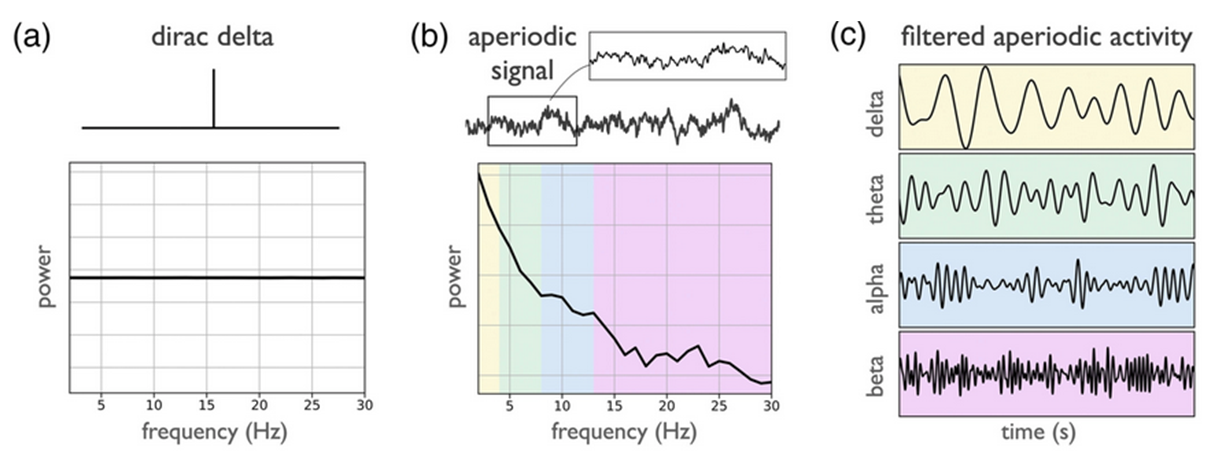
\includegraphics[scale=0.42]{11_1}
              \centering
          \end{figure}
    \item Another aspect that is crucial is that using the periodogram (either the standard version
          or the modified one by Welch), the signal is usually partitioned into different time windows of a
          given length in order to perform the Fast Fourier Transfrom (FFT) for each window, then averaging
          all of them. The time window length is defined at the beginning of the algorithm, then it runs across
          all the possible windows. If there is a signal that is constant in energy across time (such as a sinusoid),
          the duration of the window is not relevant. On the other hand, if the signal is very different from
          a sinusoid (as in the case of neuronal oscillations), the selected window acts as a low-pass filter:
          for this reason there is not an optimal way to select the window length. Ideally, the best strategy
          is to have a time-window that is dependent on the frequency taken into account, but this is not possible
          in the Fourier Analysis.
\end{enumerate}
\subsubsection{Frequency Bands}
What can be done is to concentrate the analysis in the so called \textbf{frequency peaks}.
In general, the procedure is to take the spectrum and localize the frequency range where
there is the maximum amplitude, as large increases are likely to have some sort of oscillations.
Then the analysis can be focused on that specific region of the frequency spectrum.\\
Since brain rhythms have a very neatly organized frequency distribution, the frequency
bands corresponding to those specific brain regions can be also used to separate the signals
and look at the activity. For instance, alpha peaks are considered a stable trait marker,
that can also be associated with some clinical disorders, displaying a slower frequency in
attention-deficit hyperactivity disorder (ADHD).\\
However, attention must be paid when using these frequency ranges: even if the presence of
oscillations is verified, the use of canonically defined frequency ranges may still fail
to accurately reflect the data, as this may misestimate the power of an oscillation if the
spectral peak is not well-captured in the canonical range.
\paragraph{Example} A canonically defined alpha range of \(8-12\,Hz\) captures the peak of
a \(10\,Hz\) oscillation, but fails to accurately capture an \(8\,Hz\) peak.
\begin{figure}[H]
    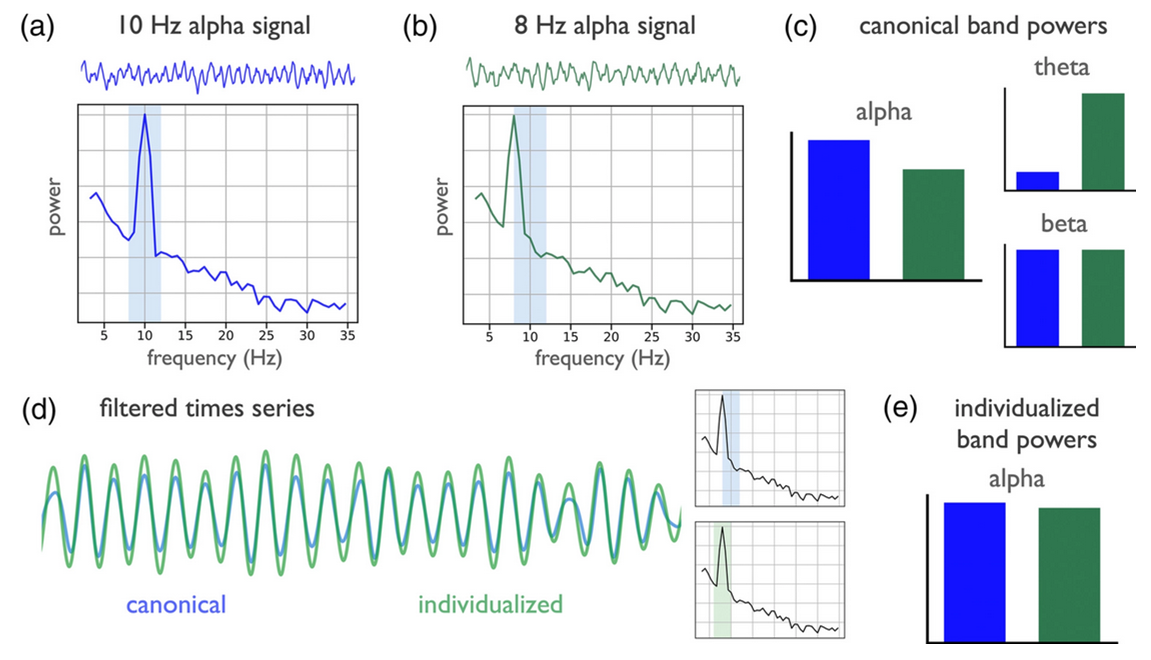
\includegraphics[scale=0.375]{11_2}
    \centering
\end{figure}
Moreover, brain oscillations are more dependent on the subject and the system itself than
on theoretical mathematical laws.\\
The Fourier Transform decomposes the signal in a weighted sum of complex sinusoids:
\begin{equation*}
    X_k=\sum_{n=0}^{N-1} x_n\cdot e^{-\frac{i2\pi}{N}\cdot kn}
\end{equation*}
Anyhow, if the signal is significantly non-sinusoidal, the neuronal oscillations are highly
non-stationary. In this way, the Fourier Transform may not be the best tool to investigate
the activity. Another possibility to characterize the activity properties is to look at the
spectrum, to define the frequency band of interest, to filter the activity there, and then go
back to the time domain and quantify what is the distance that the oscillation has from the
sinusoid. One possibility is to create a \textbf{time-resolved peak-through symmetry}
(or asymmetry), understanding how much these peak-through distances are different from a pure sine.
\subsubsection{Periodic and Aperiodic Components}
The power spectrum of a brain signal is usually distributed following a \textbf{power-law distribution},
that decays as the frequency increases at the power of an \(\alpha\) parameter, which controls the slope
of the decay.\\
There is a lot of evidence suggesting the decay depends on several physiological or pathological parameters:
for this reason, it is not considered as noise.\\
Therefore, one of the first things to do in a Fourier-based analysis is to separate the periodic
- i.e., the brain oscillations - from the aperiodic spectral components. One way is to use the
algorithm proposed by \textit{Donoghue T. et al. (2020)}, summarized in the following steps:
\begin{figure}[H]
    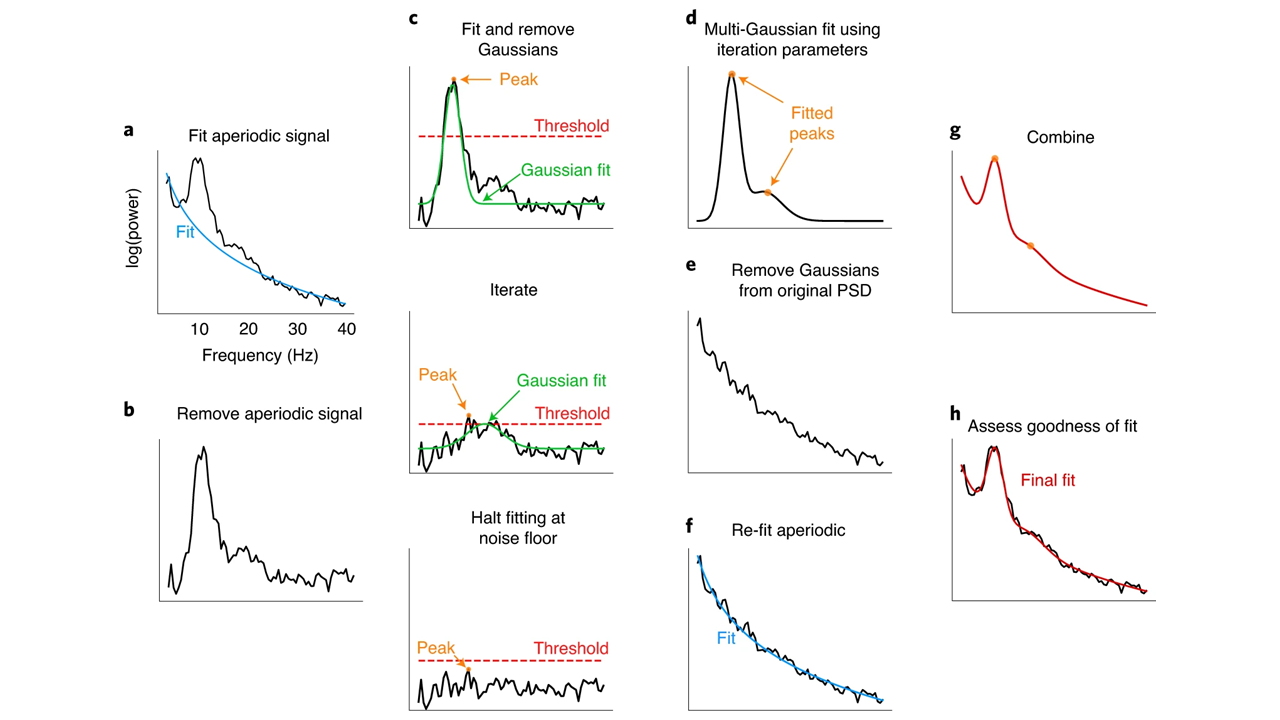
\includegraphics[scale=0.35]{11_3}
    \centering
\end{figure}
\begin{itemize}
    \item[\textbf{a.}] First, the PSD is fit with an estimated aperiodic component (blue).
    \item[\textbf{b.}] The estimated aperiodic portion of the signal is subtracted from the raw PSD, the
        residuals of which are assumed to be a mix of periodic oscillatory peaks and noise.
    \item[\textbf{c.}] The maximum peak of the residuals is found (orange). If this peak is above the noise
        threshold (dashed red line), calculated from the standard deviation of the residuals, then a Gaussian
        (solid green line) is fit around this peak based on the peak frequency, power, and estimated bandwidth.
        The fitted Gaussian is then subtracted and the process is iterated until the next identified point
        falls below a noise threshold or the maximum number of peaks is reached.
    \item[\textbf{d.}] Multi-Gaussian fitting is then performed on the aperiodic-adjusted signal (\textbf{b})
        to account for the joint power contributed by all of the putative oscillations together.
    \item[\textbf{e.}] This multi-Gaussian model is then subtracted from the original PSD (\textbf{a});
    \item[\textbf{f.}] A new fit for the aperiodic component is estimated.
    \item[\textbf{g.}] This re-fit aperiodic component is combined with the multi-Gaussian model to produce
        the final fit;
    \item[\textbf{h.}] The final fit (red) is obtained.
\end{itemize}
Another method to separate the aperiodic component from the periodic one is the
\textbf{Irregular-Resampling Auto-Spectral Analysis} (IRASA). This algorithm starts from the idea
that noise is a scale-free property of the system, while the brain oscillations are strongly dependent on the
time interval of interest. IRASA resamples the time course of the activity at different scales (both
down-sampling and up-sampling), and it repeats the Fourier Analysis at every different resampling factor.
When there is a resampling, the peak of the oscillations moves, depending on the kind of resampling. By repeating
this for multiple times and taking the median of all possible resamplings, what remains is just the
scale-free component, thus the aperiodic component itself.
\begin{figure}[H]
    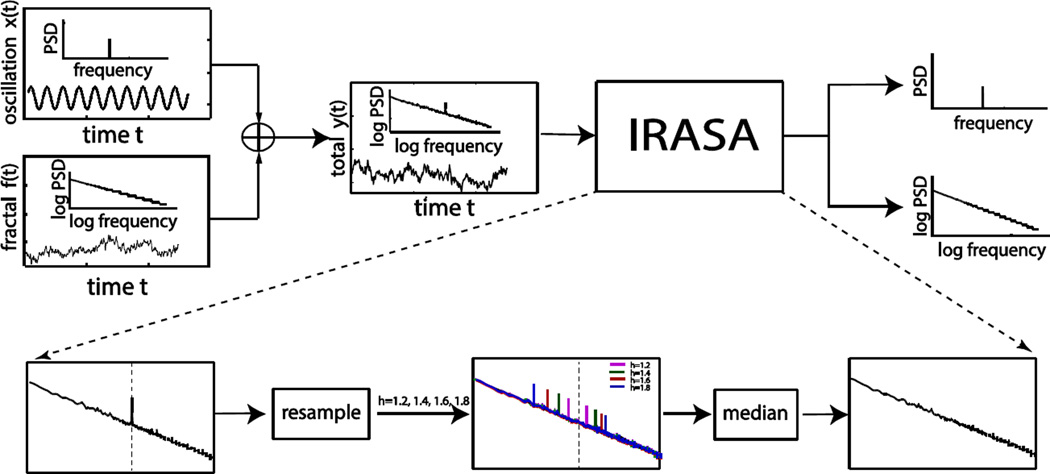
\includegraphics[scale=0.55]{11_4}
    \centering
\end{figure}
Studies have shown that the aperiodic component carries relevant information and that different behaviours
can be extracted by looking at the \(1/f\) component:
\begin{itemize}
    \item In the study of \textit{Voytek B. et al. (2020)} was found that the aperiodic exponent is linked
          to \textbf{brain maturation}: when the brain evolves from the early childhood to adulthood, the
          aperiodic exponent usually becomes less steep. This behaviour can be noticed also in the first years
          of life.
          \begin{figure}[H]
              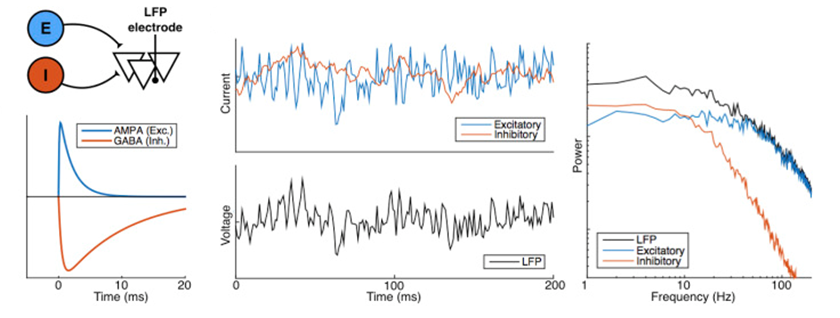
\includegraphics[scale=0.45]{11_5}
              \centering
          \end{figure}
    \item The \(1/f\) decay is also correlated with the \textbf{excitation/inhibition (\(E/I\)) balance}.
          In a study of 2017, Richard Gao created a small model of excitatory and inhibitory populations
          (that both simulated the action of pyramidal neurons). By looking separately at the excitatory
          and inhibitory components in the PSD, it is evident that the inhibitory component has a faster
          decay with respect to the excitatory one: in that sense, the aperiodic component can be used as
          a possible correlation with a larger inhibitory activity.
          \begin{figure}[H]
              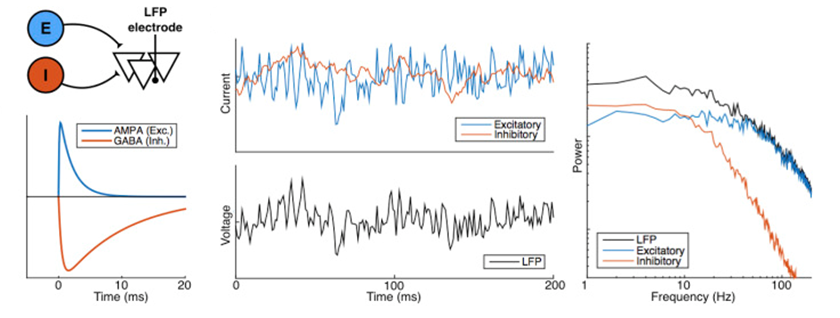
\includegraphics[scale=0.55]{11_6}
              \centering
          \end{figure}
\end{itemize}
Notice that these systems have some major drawbacks:
\begin{enumerate}
    \item If the initial field used to widen the spectrum is not accurate, then the whole analysis will be
          strongly affected by it. If at some point the decay changes its shape, as soon as the activity
          reaches the noise level of the amplifiers there is nothing that can be detected and, when the
          flattening is long enough, the initial field will be modified by this plateau. Hence, one needs to
          pay great attention to setting the parameters for the initial fitting.
    \item A particular accuracy must be paid also in selecting the resampling factors when there are multiple
          peaks of different sizes: the broad peaks require a larger sampling factor, while the thin peaks a
          smaller one. If this process is disregarded, the activity won't be completely separated.
          \begin{figure}[H]
              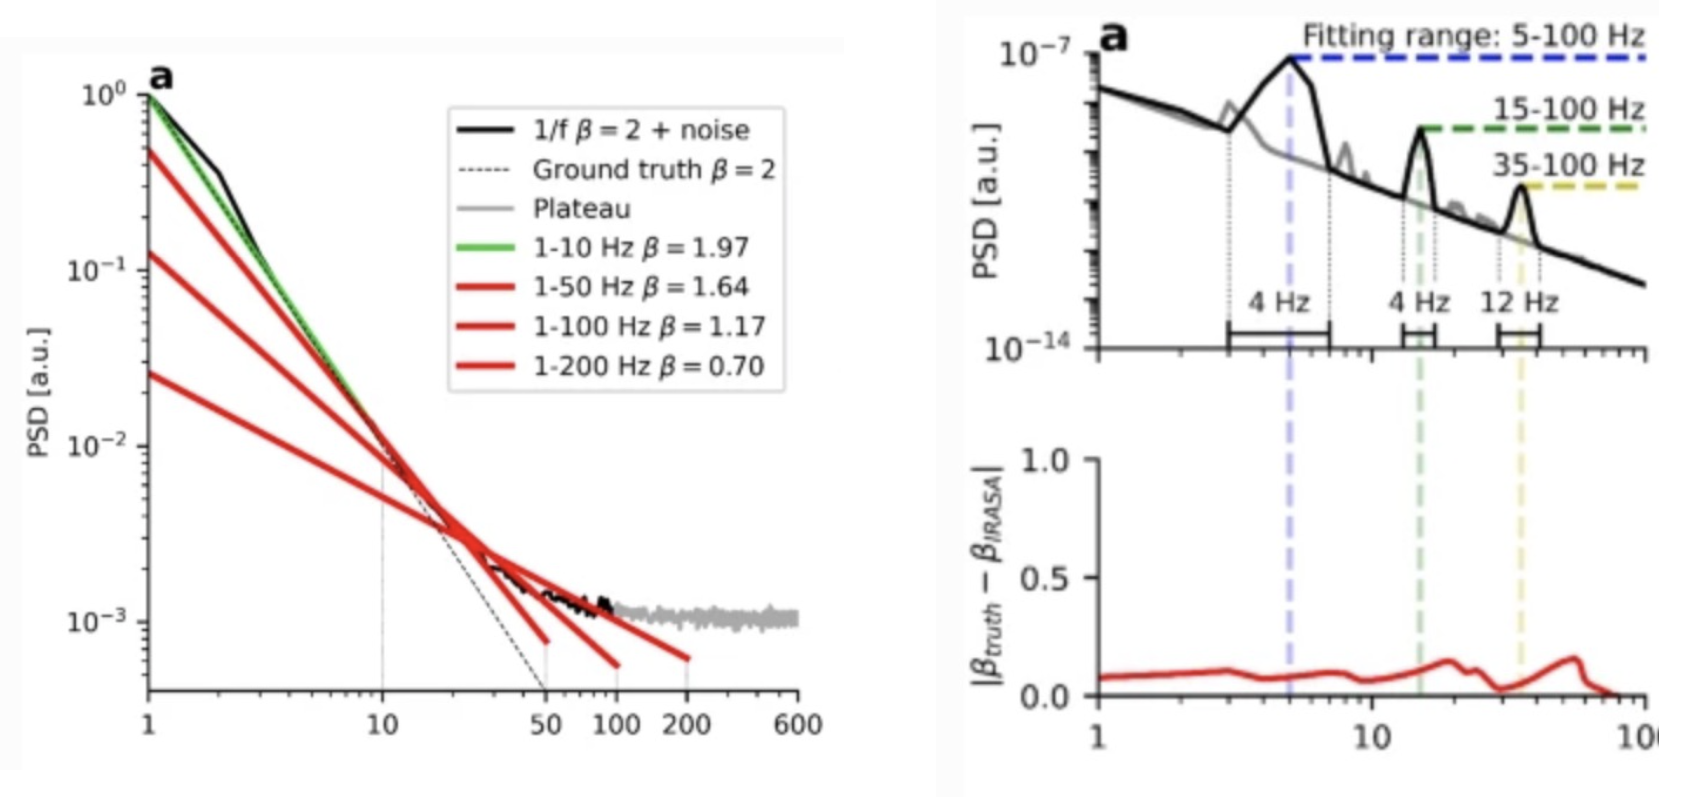
\includegraphics[scale=0.35]{11_7}
              \centering
          \end{figure}
\end{enumerate}
\subsubsection{PSDs Limitations}
By employing the Power Spectrum Density, some issues are introduced:
\begin{itemize}
    \item Brain oscillatory signals violate the stationary signal requirement of Fourier-based analysis.
    \item Fourier-based spectral decomposition can tell whether an oscillation is present or not, but
          it cannot point out when (or where) it occurs.
\end{itemize}
Is there a way to obtain a joint time-frequency representation?

\subsection{Short-Time Fourier Transform}
The \textbf{Short-Time Fourier Transform} (STFT) is one possibility to access the time-frequency decomposition.
It consists in performing the Fourier Transform for smaller time-windows of a fixed length, and then looking
at them as a 2D plot (frequency vs. time), where the third dimension - i.e., the amplitude - is given by a
colormap. Instead of separating the signal in multiple time windows and then averaging across them, the window
dimension is kept fixed and all the Fourier Transforms are aligned into time bins. The larger the time bin,
the better the frequency resolution, but at the expense of a worse temporal resolution (for the
Heisenberg Uncertainty Principle).
\begin{figure}[H]
    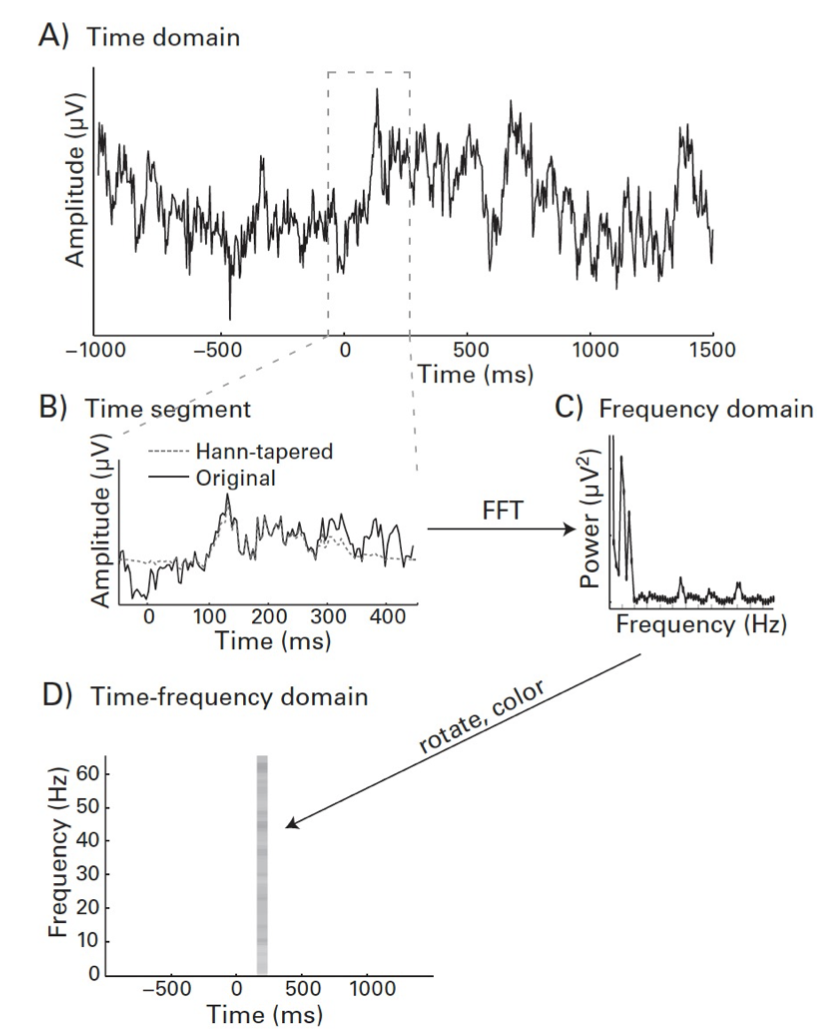
\includegraphics[scale=0.45]{11_8}
    \centering
\end{figure}
The problem of this method is that it's still Fourier-based. What can be done is to repeat the procedure for
more than one time window, adding another dimension. Anyway, this would increase the total computational cost
and the full analysis will be very complicated.
\subsubsection{Fourier Analysis Limitations}
\begin{itemize}
    \item Fourier does not provide temporal information on discrete increase of amplitude of an oscillation
          (sine is always the same across time).
    \item Fixed widths for time windows in STFT creates a problem in neuroscience, since signals need to be
          stationary in order to be able to apply the Fourier theorem, but neural signals are non-stationary.
\end{itemize}

\subsection{Wavelet Transform}
\subsubsection{Convolution Theorem and Wavelet Transforms}
As described before, what the Fourier Transform does is filtering the signal with a sine wave for multiple
frequencies, through a dot product or a convolution. The dot product can be interpreted mainly in two ways:
\begin{itemize}
    \item as a filtering process in which a filter with a given kernel is applied to the signal at multiple
          time instants. The most used kernels are composed of single sine waves with different frequencies.
    \item as a time correlator between two signals (from a statistical/geometrical point of view).
\end{itemize}
Nonetheless, such an approach does not allow to separate time from frequency: a joint time-frequency
representation cannot be obtained.
\begin{figure}[H]
    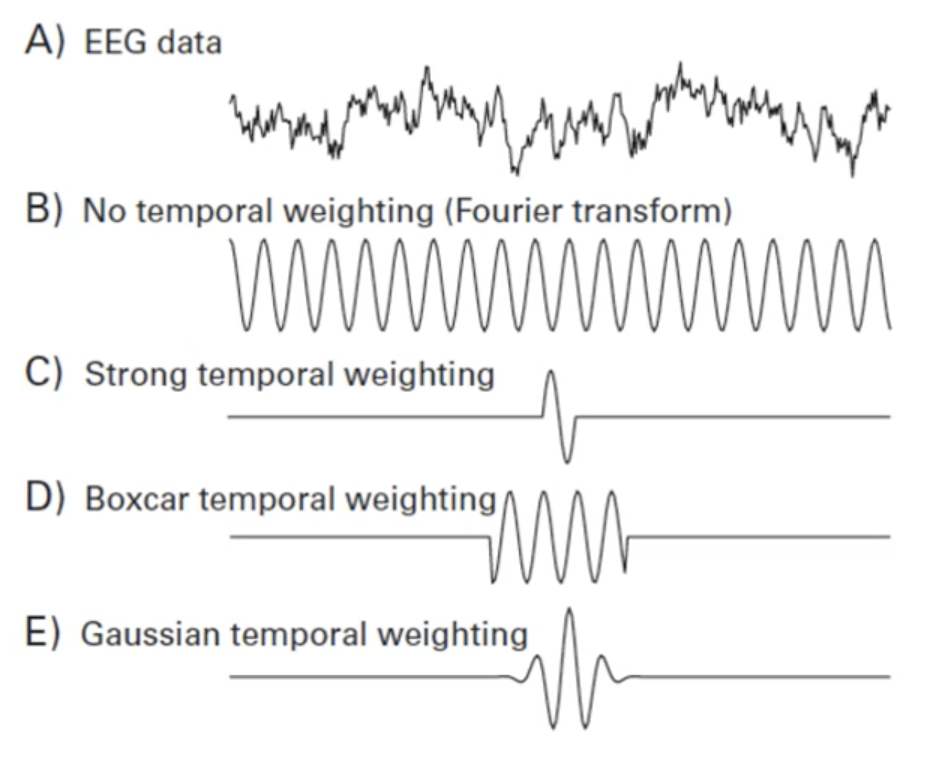
\includegraphics[scale=0.35]{11_9}
    \centering
\end{figure}
One possibility to access the time resolution would be to filter the EEG data through a narrow temporal window.
For instance, the \textbf{C} window presented in the picture above can be used: in this case a stronger
correlation in the central part of the signal can be expected (the profile is similar). However, even if this
window would allow a very high temporal resolution, it would also create a very broad frequency spectrum - i.e.,
low frequency resolution -.\\
The opposite possibility would be applying a boxcar temporal weighting such as \textbf{D}, that would access a
larger frequency resolution but also cause a reduced temporal resolution.\\
However, in bot cases borders would affect negatively the whole structure. To remove this problem, a Gaussian
window can be used. Multiplying it by a complex sine wave, a \textbf{Gabor wavelet} or a
\textbf{Morlet wavelet} is obtained.
\begin{figure}[H]
    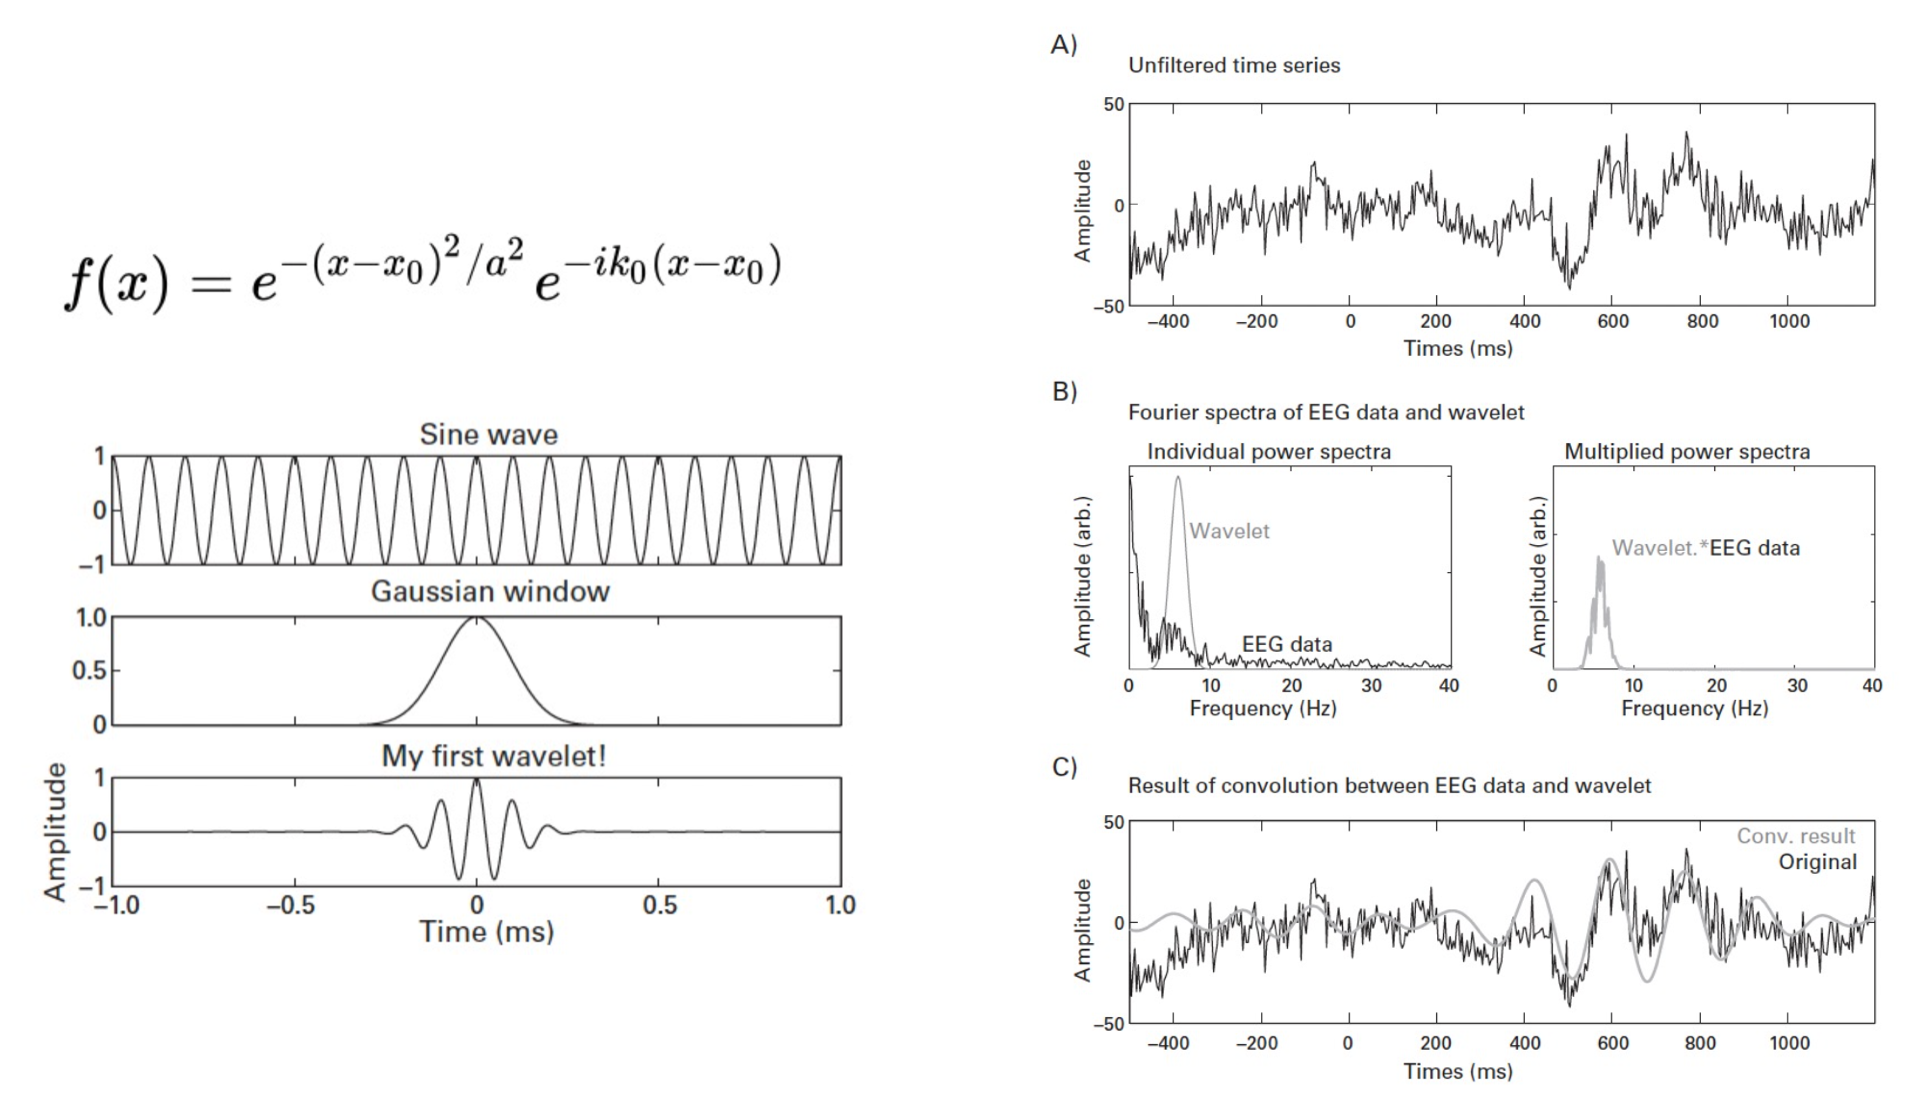
\includegraphics[scale=0.4]{11_10}
    \centering
\end{figure}
The Gaussian function is also the best one in reducing the trade-off between
temporal and spectral resolutions: high time and frequency resolutions can be accessed in a much more efficient
way compared to Fourier Transforms.\\
The advantage of using a Gabor function can be explained by remembering that the transform of a sine is an
impulse and the one of a Gaussian is still a Gaussian. Thus, by performing the convolution of the Gabor wavelet
and the initial signal, a filter in a very specific frequency range is obtained. The position of this filter
can be controlled through the main frequency of the sine wave and its bandwidth through the variance of the Gaussian.\\
Through the combination of multiple wavelets, the EEG signal can be decomposed into a time-filtered signal
with zero mean, which captures really well the sinusoidal components by increasing the amplitude of the filtered
signal.
\subsubsection{Real-Valued vs Complex Wavelets}
The complex wavelet is not the only one that exists, but it is important for two reasons:
\begin{enumerate}
    \item If only real-valued wavelets are considered, if the two oscillations that need to be matched are not
          aligned in phase, the dot product will be affected by it. Hence, complex wavelets are more
          complicated, but have the advantage that for them the phase is one of the parameters. Thus, they
          allow a more general representation, accounting for all possible shifts.
    \item Complex wavelets enable also the separation of the amplitude dynamics from the phase dynamics of the
          signals, such that the two aspects can be analyzed separately.\\
          Spectral coherence is dependent both on phase differences and on amplitude correlations, so when looking
          at an increased spectral coherence one cannot immediately deduce which factor influenced it.
          Analyzing the signal by using complex wavelet components allows to understand whether the property
          that is being considered is more dependent on amplitude correlation or phase synchronization.
\end{enumerate}
\begin{figure}[H]
    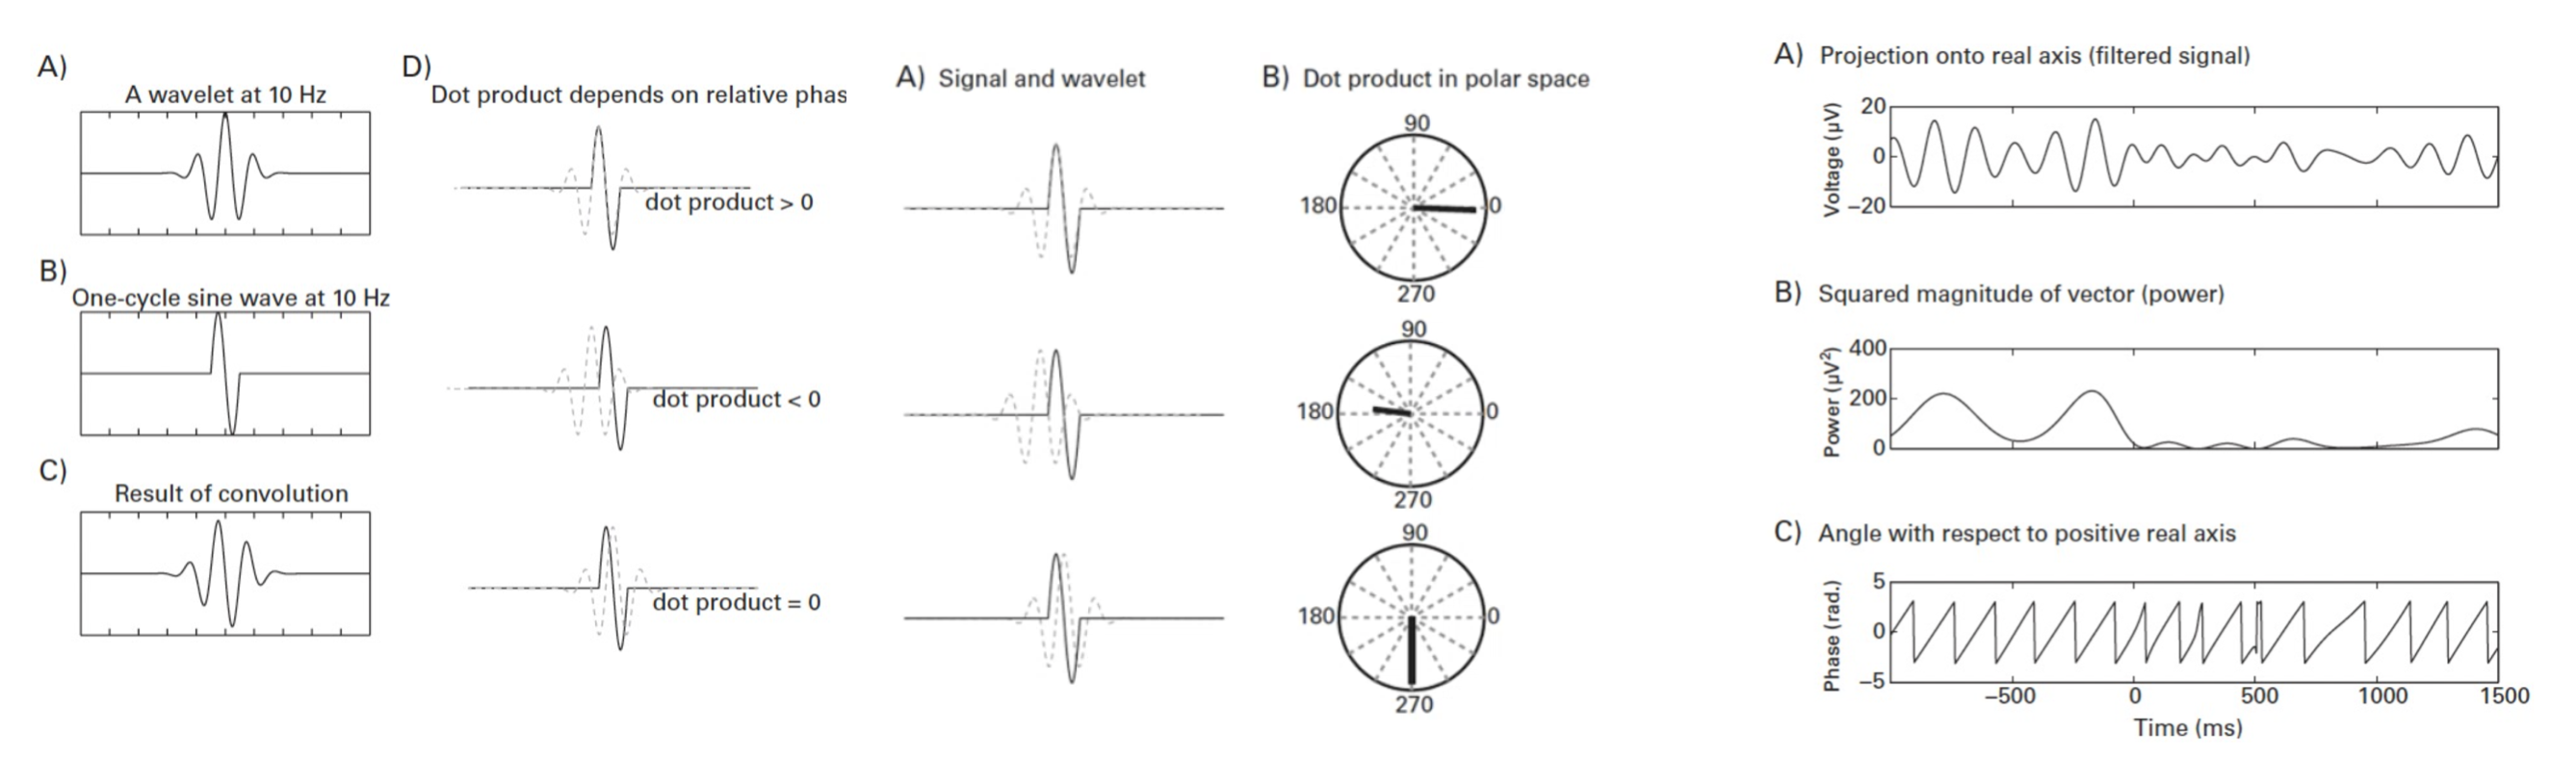
\includegraphics[scale=0.35]{11_11}
    \centering
\end{figure}
\subsubsection{Frequency Scale and Resolution}
In general, an optimal frequency range does not exist, unless the modulation of a specific kind of wave is
considered.
\begin{itemize}
    \item \textbf{Minimum frequency:} usually dictated by the experimental conditions and by the length of the
    data. In the resting state there is no limit to the minimum frequency, apart from going below \(1\,Hz\)
    of frequency oscillations, that requires dedicated hardware. Short windows act as high-pass filters.
    \item \textbf{Maximum frequency:} limited by the Nyquist theorem.
\end{itemize}
About the frequency scale - i.e., how many and how spaced frequencies must be - there is no fixed optimal
decision either. It is usually dictated by the visualization of the results and on whether slow or fast
oscillations are considered:
\begin{itemize}
    \item \textbf{Faster rhythms:} require a logarithmic kind of representation (better visual resolution).
    \item \textbf{Slower rhythms:} require linear, highly sampled frequencies.
\end{itemize}
Even a combination of the two can be used, but it would be hard to read in terms of visual results.
\begin{figure}[H]
    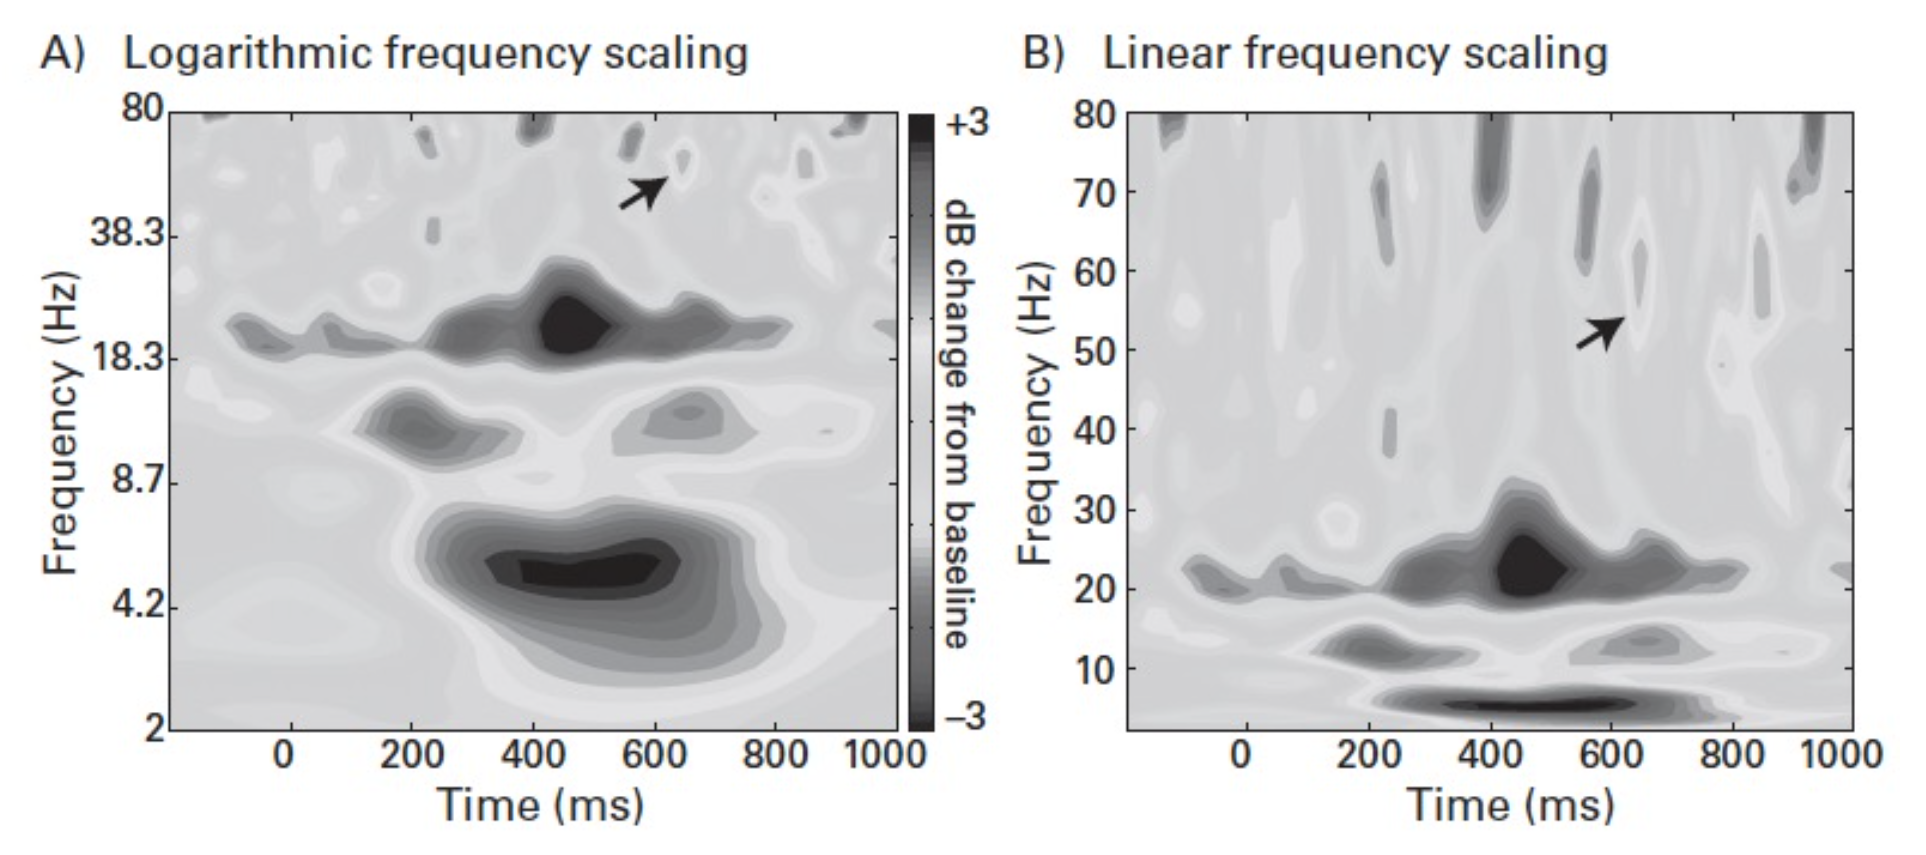
\includegraphics[scale=0.35]{11_12}
    \centering
\end{figure}
\subsubsection{Time Scale and Resolution}
The selected kernel should be long enough to contain at least some cycles of the sine wave, but not too long
to suppress all the oscillations. Therefore, the time window of the filter needs to reach 0 in a smooth way
as fast as possible, but at the same time to contain enough cycles of oscillation, because the Heisenberg
Uncertainty Principle applies here.
resolutions.
\begin{figure}[H]
    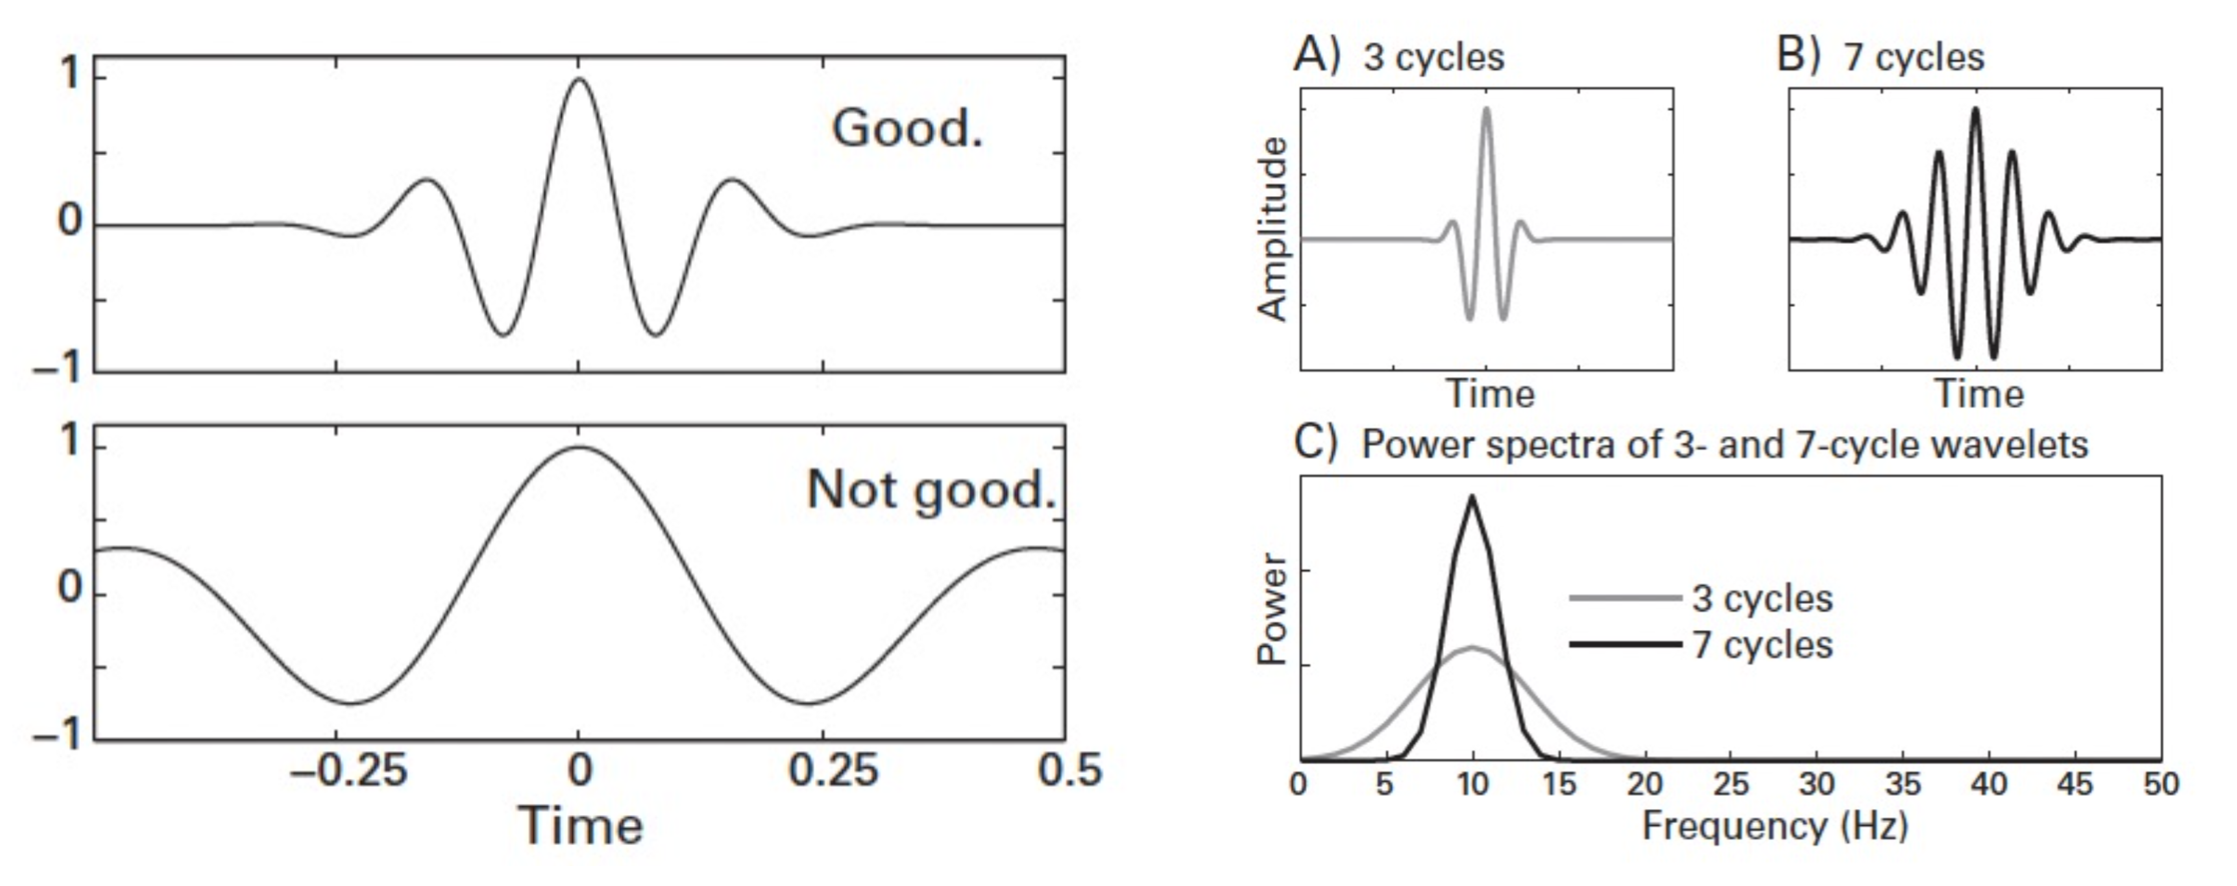
\includegraphics[scale=0.3]{11_13}
    \centering
\end{figure}
The number of cycles is identified as the number of peaks inside the
wavelet. The power spectrum of the different wavelets is again a Gaussian that is centered around 0 and both
reach 0 at the same time, but the variance is different in the two cases: one has a smaller frequency
resolution, while the other one is wider. The \(3\) cycles wavelet gives a better time resolution, while the
frequency will be smoother in a wider region. For the \(7\) cycles wavelet, the frequency resolution is better, on
the contrary the time resolution is worse.\\
An optimal trade-off for neuroscience is in the range of \(5-7\) cycles to have accurate frequency and time
resolutions.
